% Пример статьи для журнала КИО

\documentclass[eqsecnum,authorsinfo]{kioj6}


% Здесь можно подключить свои пакеты.
\usepackage{enumitem}
\usepackage{tabularray}

% ========== НАСТРОЙКИ СПИСКА ЛИТЕРАТУРЫ ==========
%
% \newcommand{\bibfontsize}{\footnotesize}   % размер шрифта в библиографии
% \newcommand{\biblinespread}{1.1}            % межстрочный интервал внутри записи
% \newcommand{\bibitemsep}{0pt}               % вертикальный отступ между записями


% ========== НАСТРОЙКИ ДЛЯ ПРЕДОТВРАЩЕНИЯ ВИСЯЧИХ СТРОК ==========
%\raggedbottom  
%\widowpenalty=10000
%\clubpenalty=10000

% ===================== НАСТРОЙКИ ЖУРНАЛА ====================

% Указываем номер страницы, с которой начинается статья
\setcounter{page}{2}

% Рубрика в журнале (не всегда известна при подаче статьи)

%\journalsectionnoimage{algorithmic-mathematics}
%\journalsectionnoimage{artificial-intelligence}
%\journalsectionnoimage{informatics}
%\journalsectionnoimage{information-systems}
%\journalsectionnoimage{software-engineering}
%\journalsectionnoimage{computer-in-education}
%\journalsectionnoimage{popular-science-articles}
%\journalsectionnoimage{programming-practice}
%\journalsectionnoimage{editorial-column}
%\journalsectionnoimage{specialists-training-new-teaching-methods}
%\journalsectionnoimage{specialists-training-training-programs}
%\journalsectionnoimage{specialists-training-professional-standards}
%\journalsectionnoimage{open-problems-for-young-scientists}
\journalsectionnoimage{empty}

% Указывам год, номер выпуска неизвестен, поэтому ставим прочерк, указываем edu, что означает журнал "Компьютерные инструменты в образовании".

\issue{2026}{--}{edu}

% ===== ТИП СТАТЬИ ====
% 1. {1}  → Исследовательская статья / Research article
% 2. {2}  → Обзорная статья / Review article
% 3. {3}  → Материалы конференции / Conference paper
% 4. {4}  → Редакционная статья / Editorial article
% 5. {5}  → Дискуссионная статья / Discussion article
% 6. {6}  → Краткое сообщение / Short Communication

\articletype{1}


\udknumber{999.999}
\doinumber{10.32603/2071-2340-2026-4-XXX-XXX}

% =============== ДАННЫЕ НА РУССКОМ ЯЗЫКЕ ===============

% Заголовок статьи (русский)
\title[К вопросу об оформлении научных статей]{К вопросу об оформлении научных статей с~использованием современных технических средств на~основе пакета прикладного ПО \LaTeX}

% Авторы (русская версия)
\author{1}[Андреев А.~А.\affil{1,3}]{Андреев Аркадий Александрович}
\authorinfo{1}{д. ф.-м. н., профессор кафедры алгоритмической математики факультета компьютерных технологий и информатики СПбГЭТУ «ЛЭТИ»}
\authororcid{1}{orcid.org/0000-0000-9999-9999}
\authoremailEnvelope{1}{aaandreev@etu.ru} % адрес для корреспонденции

\author{2}[Богоявленский-Мелитопольский М. М.\affil{2}]{Богоявленский-Мелитопольский Максим Маратович}
\authorinfo{2}{к. ф.-м. н., н. с. Лаборатории радиоастрономических наблюдений ИПА РАН}
\authoremail{2}{mbm@iaaras.ru}

\author{3}[Воронов В.~В.\affil{3}]{Воронов Владимир Владимирович}
\authorinfo{3}{аспирант, ассистент факультета математики и компьютерных наук СПбГУ}
\authoremail{3}{v.v.voronov@spbu.ru}

\author{4}[Ге В.~Г.\affil{4}]{Ге Вильгельмина Геннадьевна}
\authorinfo{4}{руководитель отдела контроля качества компании «Квантори»}
\authororcid{4}{orcid.org/0000-9999-9999-9999}
\authoremail{4}{vilgelmina.g.ge@quantori.com}

% Аффилиации
\affiliation{1}{Санкт-Петербургский государственный электротехнический университет «ЛЭТИ»,
  ул. Профессора Попова, 5, 197022, Санкт-Петербург, Россия}
\affiliation{2}{Федеральное государственное бюджетное учреждение науки
  Институт прикладной астрономии Российской академии наук, наб. Кутузова, 10, 191187, Санкт-Петербург, Россия}
\affiliation{3}{Санкт-Петербургский государственный университет,
  Университетская набережная, д. 7–9, 199034, Санкт-Петербург, Россия}
\affiliation{4}{Quantori LLC, 1 Broadway, Cambridge, MA 02142, United States}

% ========== ДАННЫЕ НА АНГЛИЙСКОМ ЯЗЫКЕ ==========

% Заголовок статьи (английский)
\titleen[On typography of scientific articles]{On typography of scientific articles using modern tools based on software from the \LaTeX\ family}

% Авторы (английская версия)
\authoren{1}[Andreev A.~A.\affil{1,2}]{Andreev Arkady Aleksandrovich}
\authorinfoen{1}{D. Sc., professor at the Department of Algorithmic Mathematics, Faculty of Computer Technology and Informatics, ETU ``LETI''}

\authoren{2}[Bogoyavlenskiy-Melitopolskiy M.~M.\affil{2}]{Bogoyavlenskiy-Melitopolskiy Maksim Maratovich}
\authorinfoen{2}{Ph. D., researcher at the Laboratory of radioastronomical observations, IAA RAS}

\authoren{3}[Voronov V.~V.\affil{3}]{Voronov Vladimir Vladimirovich}
\authorinfoen{3}{postgraduate student, assistance lecturer at the Faculty of Mathematics and Computer Science, SPbSU}

\authoren{4}[Ge V.~G.\affil{1,3}]{Ge Vilgelmina Gennadievna}
\authorinfoen{4}{Head of Quality Assurance, Quantori LLC}

% Аффилиации (английские)
\affiliationen{1}{Saint Petersburg State Electrotechnical University, Professora Poposa st.,, 5, 197022, St. Petersburg, Russia}
\affiliationen{2}{Institute of Applied Astronomy of the Russian Academy of Sciences, Kutuzova emb. 10, 191187, St. Petersburg, Russia}
\affiliationen{3}{Saint Petersburg State University, Universitetskaya emb. 7--9, 199034, St. Petersburg, Russia}
\affiliationen{4}{Quantori LLC, 1 Broadway, Cambridge, MA 02142, United States}

\begin{document}

	% ========== РУССКАЯ ЧАСТЬ ==========

	\russianversion
	\maketitle
	\pagestyle{mainstyle}

	\begin{abstract}
	  Используйте данный образец при подготовке статей в журнале <<Компьютеpные инструменты в образовании>>.
          В образце приведены примеры оформления разделов, подразделов, списков, таблиц, формул и ссылок на все эти сущности,
          а также примеры ссылок на библиографические источники, заданные в виде файла формата Bibtex.

          Аннотация должна кратко описывать контекст, методы и результаты исследования. Чтение статей происходит
          обычно в следующем порядке: название, авторы, аффилиации авторов, аннотация, результаты в конце --- и
          лишь после этого, если читатель заинтересовался, он начинает читать разделы статьи, начиная с Введения.
          
          В аннотации допустимы абзацы и, при необходимости, внутритекстовые формулы ($e^{i\pi} + 1 = 0$), но
          не допускаются ссылки на элементы статьи и на источники.
          
	  \keywordsru{Оформление, Латех, Бибтех}
	  \autocitation
          % Или ручное цитирование: \manualcitation{text}
	\end{abstract}

    \section{Введение}
    Жуpнал <<Компьютеpные инстpументы в обpазовании>> выходит с января 1998 года.
    Научное направление периодического издания: алгоритмическая математика и математическое моделирование, информатика и информационные технологии, автоматизация процессов в области образования.
    
    Исторически журнал сложился как общее пространство для обсуждения
    проблем, связанных с обогащением обучения математике и информатике
    за счет использования компьютерных инструментов.  В связи с тем,
    что в современных условиях использование компьютерных инструментов
    начинает непосредственно влиять на сам предмет математики, журнал
    все большее внимание уделяет компьютерной математике и
    информатике.  Большое внимание журнал уделяет донесению актуальных
    исследований до студентов, поэтому привествуются статьи,
    разъясняющие новые идеи информатики и алгоритмической математики и
    статьи с постановкой задач для молодых ученых.

    Введение должно содержать описание темы исследования и обзор
    предыдущих работ, посвящённых этой или смежным темам.

    \section{Примеры форматирования текста}\label{sec:formatting}
    Заголовки первого уровня отображаются в верхнем регистре, но перевод в верхний регистр происходит автоматически,
    делать это в исходном коде не нужно. (Благодаря этому название раздела останется в обычном регистре в оглавлении
    PDF-файла.).
    
    Приведём пример нумерованного списка. Обратите внимание на пунктуацию.
    \begin{enumerate}
        \item Первый пункт;
        \item Второй пункт;
        \item Третий пункт.
    \end{enumerate}

    \subsection{Изображения}\label{sec:images}
    Обычное (одиночное) растровое изображение, снабжённое подписью, приведено на рис.~\ref{fig:example}.

    \begin{figure}[htb]
        \centering
        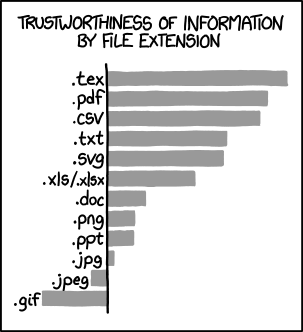
\includegraphics[width=0.3\textwidth]{xkcd1301.png}
        \caption{Достоверность информации в зависимости от расширения файла} \label{fig:example}
    \end{figure}

    \subsubsection{Составные изображения}

    Рис.~\ref{fig:example-2} содержит два векторных изображения: \ref{fig:example-2a} и \ref{fig:example-2b}.
    
    \begin{figure}[H]
        \centering
        \begin{subfigure}[t]{70mm}
             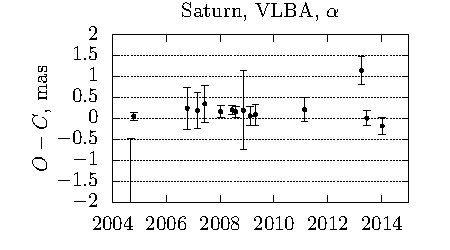
\includegraphics{saturn-vlba-alpha.pdf}
         \subcaption{Необязательный подзаголовок}
         \label{fig:example-2a}
        \end{subfigure}
        \ %это пробел между двумя рисунками
        \begin{subfigure}[t]{70mm}
         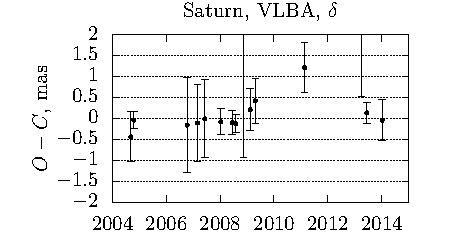
\includegraphics{saturn-vlba-delta.pdf}
            \subcaption{} % Здесь подзаголовок не указан
            \label{fig:example-2b}
        \end{subfigure}
        \caption{Пример двух изображений рядом на одном рисунке} \label{fig:example-2}
    \end{figure}
    
    \subsection{Таблицы}

    \subsubsection{\texttt{tabular}}
\begin{table}[ht]
  \centering
\caption{Солнечные штормы классов G3-G5 в 2024 г. с датой прогноза и датой и временем прихода ударной волны}
\label{tbl:events}
\begin{tabular}{|c|c|c|} \hline
  Ранжирование по Dst,   & Дата     & Время прихода            \\
  G-индекс               & прогноза &  ударной волны \\ \hline
  \#1 (G5) & 2024-05-10 & 2024-05-11T11  \\ \hline
  \#2 (G5) & 2024-05-09 & 2024-05-10T17  \\ \hline 
  \#3,4 (G4--3) & 2024-10-09 & 2024-10-11T15  \\ \hline 
  \#6 (G3) & 2024-05-10 & 2024-05-12T10  \\ \hline 
  \#5,9 (G4) & 2024-08-10    & 2024-08-11T07  \\ \hline
  \#7 (G3) & 2024-10-06 & 2024-10-06T08  \\ \hline 
  \#8 (G4) & 2024-03-23 & 2024-03-24T15 \\ \hline
  \#10 (G3) & 2024-04-18 & 2024-04-19T06 \\ \hline
  \#11 (G4) & 2024-09-14 & 2024-09-16T23\\ \hline
  \#12 (G3) & 2024-08-01 & 2024-08-04T15 \\ \hline
  \#13 (G3) & 2024-09-10 & 2024-09-12T04\\ \hline
  \#15 (G4) & 2024-06-25 & 2024-06-28T11\\ \hline 
\end{tabular}
\end{table}
    
    \subsubsection{\texttt{tblr}}
    \begin{table}[H]
  \centering
  \caption{Пример сложной таблицы}
  \label{tbl:complex}      
\begin{tblr}{
  hlines, vlines, % borders around each cell
  rowsep=0pt, colsep = 0pt,
  rows = {20pt}, columns = {100pt}, % fixed width columns and fixed height rows
  cells = {c,m}, % centered cells (vertically and horizontally)
  cell{1}{1} = {r=2}{}, % multirow
  cell{1}{2} = {c=2}{}, % multicolumn
}
State of Health & Fasting Value &         & After Eating         \\
                & Minimum       & Maximum & 2 hours after eating \\
Healthy         & 70            & 100     & Less than 140        \\
Pre-Diabetes    & 101           & 126     & 140 to 200           \\
Diabetes        & More than 126 & N/A     & More than 200        \\
\end{tblr}
\end{table}

    \subsection{Формулы}

    Ур-е~(\ref{eq:gaussian}) --- нумерованное, потому что на него есть ссылка в тексте.
    
    \begin{equation}
        \int_{-\infty}^{\infty} e^{-x^2} \, \mathrm{d}x = \sqrt{\pi}
        \label{eq:gaussian}
    \end{equation}
    
    Выключные формулы могут быть и ненумерованными, например:

    $$\frac{d}{dt} \left( \frac{\partial L}{\partial \dot{\symbfit{q}}} \right) = \frac{\partial L}{\partial \symbfit{q}},$$

\noindent где $L$ --- Лагранжиан, $\symbfit{q}$ --- обобщённые координаты, $\dot{\symbfit{q}}$ --- обобщённые скорости.
    

    \section{Примеры ссылок}
    Ссылка на разд.~\ref{sec:formatting}.

    Далее приведены ссылки на различные типы источников. Для каждого
    типа приведены один-два примера: их можно использовать как образец
    оформления и удалить из итоговой статьи.

    Источники хранятся в файлах
    \texttt{references.bib} и \texttt{references-en.bib} (второй файл --- только
    для англоязычных аналогов русскоязычных источников, присутствующих в первом файле).
    Если источник в \texttt{references.bib} изначально англоязычный, его \textit{не нужно} повторять
    в \texttt{references-en.bib}.
    
    \begin{enumerate}
        \item \textbf{Книги и главы} 
        \begin{itemize}[nosep]
            \item Книга на английском с переводом на русский~---~\cite{Hairer}.
            \item Книга на русском без английского перевода~---~\cite{Gubanov}.
            \item Глава в книге на русском без перевода~---~\cite{layexpl7}.
            \item Глава книги с указанием издания, главы, раздела и страниц~---~\cite{ogura}.
            \item Книга нескольких авторов с многими редакторами~---~\cite{HastieTibshiraniFriedman2009}.
            \item Глава с многими авторами, редактором и изданием~---~\cite{Alberts2014CellCycle}.
            \item Глава, написанная редактором тома~---~\cite{Gowers2008LanguageGrammar}.
            \item Глава с переводчиком~---~\cite{Aleksandrov1963GeneralView}.
        \end{itemize}

        \item \textbf{Статьи}
        \begin{itemize}[nosep]
            \item Статья на русском с английским переводом~---~\cite{Matveenko}.
            \item Статья в журнале с идентификатором (Art.~no.)~---~\cite{Abbott2016GW150914}.
        \end{itemize}

        \item \textbf{Блог}~---~\cite{Dmitry2024Python}

        \item \textbf{Доклад на конференции без публикации в сборнике}~---~\cite{Caratelli}.

        \item \textbf{Статья в трудах конференции}~---~\cite{BYSIS2022}

        \item \textbf{Набор данных (датасет)}~---~\cite{pavlov_2025_14923680}.

        \item \textbf{Руководство}
        \begin{itemize}[nosep]
            \item Печатное руководство (Manual)~---~\cite{TransmissionSystems}.
            \item Электронное руководство~---~\cite{BreimannRF}.
        \end{itemize}

        \item \textbf{Лекционные материалы}~---~\cite{BarneyLecture}.

        \item \textbf{Новостная статья}~---~\cite{MarkoffNews}.

        \item \textbf{Онлайн видео}
        \begin{itemize}[nosep]
            \item Видеоролик на YouTube~---~\cite{mtaOnlineVideo}.
            \item Видеоролик на VK Video~---~\cite{vkVideoExample}.
        \end{itemize}

        \item \textbf{Патент}
        \begin{itemize}[nosep]
            \item Патент~--- \cite{WilkinsonPatent}.
            \item Российский патент~---~\cite{sviridov}.
        \end{itemize}

        \item \textbf{Программное обеспечение}
        \begin{itemize}[nosep]
            \item Программное обеспечение~---~\cite{ArningSoftware}.
            \item Российское программное обеспечение~---~\cite{schoolPassportSoftware}.
        \end{itemize}

        \item \textbf{Стандарты}
        \begin{itemize}[nosep]
            \item Стандарт IEEE со всеми полями (адрес, дата, DOI, URL)~---~\cite{StdIEEE754Full}.
            \item Российский ГОСТ~---~\cite{gostMed57647}.
        \end{itemize}

        \item \textbf{Магистерская ВКР}~---~\cite{TemirgalievThesis}.

        \item \textbf{Кандидатская/PhD-диссертация}~---~\cite{MirtichPhD}.

        \item \textbf{Документ правительства}~---~\cite{DEI_Trump}.

        \item \textbf{Технический отчет}~---~\cite{DE430}.

        \item \textbf{Препринт arXiv}~---~\cite{UrazhdinArxiv}.
 
        \item \textbf{Веб-сайт}~---~\cite{ETU}.

        \item \textbf{Социальные сети}~---~\cite{ClarksonX}.
    \end{enumerate}

    \section{Заключение}
    Ваше заключение.

    \acknowledgmentsru{Авторы благодарят коллег за полезные обсуждения.}
    \fundingru{Работа выполнена при финансовой поддержке гранта №~XX-XX-XXXXX.}
    \conflictofinterestru{Авторы заявляют об отсутствии конфликта интересов.}

    \bibliographystyle{ugost2008}
    \bibliography{references-clones}

    \additionalinfo{Поступила в редакцию 7 октября 2025, окончательный вариант 28 января 2026 г.}

    \printauthorsinfo

    % ========== ПЕРЕВОДНАЯ ЧАСТЬ (на английском) ==========
    \begin{translatedpart}
        \maketranslatedtitle

        \begin{abstract}
            English abstract goes here.
            \keywordsen{keywords1, keywords2, keywords3}

            \autocitation
            %Или ручное цитирование: \manualcitation{text}
        \end{abstract}

        \begin{otherlanguage*}{english}
            \bibliographystyleeng{IEEE}
            \bibliographyeng{references-en-prefixed,references-clones}
        \end{otherlanguage*}

        \acknowledgmentsen{The authors thank their colleagues for fruitful discussions.}
        \fundingen{The work was supported by grant No.~XX-XX-XXXXX.}
        \conflictofinteresten{The authors declare no conflict of interest.}

        \additionalinfo{Received October 7, 2025, The final version: January 28, 2026}

    \end{translatedpart}
    
\end{document}
